\section{The partitioning of transmembrane current}\label{part}

Further progress requires expressions for $I_\mathrm{P}$ and
$I_\mathrm{D}$ in terms of the biophysical and morphological
properties of the segment and the membrane potentials at its
proximal and distal boundaries. Each component of the
transmembrane current (\ref{tc2}) is examined separately.

\subsection{Point processes}\label{PointInput}

We model synaptic current by the conventional constitutive
equation $\mathcal{I}=g(t)(V-E)$ where $E$ is the reversal
potential associated with the synapse and $g(t)$ is the time
course of the synaptic conductance. Exogenous point current input
takes the form $\mathcal{I}=\mathcal{I}(t)$ where $\mathcal{I}(t)$
is a known function of $t$. Suppose that $\lambda_1,\
\cdots,\lambda_n$ are sites of point input $\mathcal{I}_1,\
\cdots\ \mathcal{I}_n$ to the segment, then it follows from
expressions (\ref{potc3}) that the contributions made to
$I_\mathrm{P}$ and $I_\mathrm{D}$ from these currents are
\begin{equation}\label{ei1}
I_\mathrm{P} = \sum_{k=1}^n\,
\frac{r_\mathrm{P}}{r_k}\,(1-\lambda_k)\,\mathcal{I}_k\,,\qquad
-I_\mathrm{D} = \sum_{k=1}^n\,
\frac{r_\mathrm{D}}{r_k}\,\lambda_k\,\mathcal{I}_k
\end{equation}
where $r_k=(1-\lambda_k)\,r_\mathrm{P} +\lambda_k\,r_\mathrm{D}$.
In the special case of exogenous input alone,
$\mathcal{I}_k=\mathcal{I}_k(t)$ and expressions (\ref{ei1}) give
the exact partitioning of this input. The procedure used by the
anonymous reviewer (see Section \ref{assertion}) is an application
of equations (\ref{ei1}) to a uniform segment, that is,
\begin{equation}\label{ei11}
I_\mathrm{P} = \sum_{k=1}^n\,
(1-\lambda_k)\,\mathcal{I}_k\,,\qquad -I_\mathrm{D} =
\sum_{k=1}^n\, \lambda_k\,\mathcal{I}_k\,.
\end{equation}
However, when synaptic input is present, expressions (\ref{ei1})
for $I\mathrm{P}$ and $I_\mathrm{D}$ will contain the (unknown)
membrane potentials at the synapses, and its use will therefore
require these potentials to be estimated in terms of known
functions and the potentials at the proximal and distal boundaries
of the segment.

One obvious way to estimate the potential at the site of a synapse
is to use the potential distribution (\ref{mp3}). However, the
efficacy of this approximation relies on the validity of the
assumption that transmembrane current is negligible by comparison
with axial current. In the presence of synaptic input,
transmembrane current need not be negligible by comparison with
axial current, and so the partitioning rule must be developed to
include this possibility.

\subsection{The partitioning rule in the presence of synaptic input}\label{stage1}

The partitioning of point process input set out in Subsection
\ref{PointInput} is developed by noting that this rule may be
applied to the division of transmembrane current between
nearest-neighbour sites of a point input, and that the proximal
and distal boundaries of the segment are simply special cases of
these sites. This application of the partitioning rule is
equivalent to considering the balance between axial current and
point current at each site of input ignoring the influence of
distributed transmembrane current between sites. The
implementation of the partitioning rule for general point process
input is done in two stages. The first stage of the discussion
focusses on the construction of the equations satisfied by the
potentials at the sites of the point input, and the second stage
of the discussion describes how these equations may be solved
numerically and is contained in appendix one.

\subsubsection{Equations for the potentials}

In general, the locations of point process input can be taken to
divide a segment into sub-segments, defined to be the lengths of
the segment between the locations of these inputs. Figure
\ref{synapses} is a schematic representation of a segment of
length $h$ illustrating the relative locations $\lambda_1,\
\cdots, \lambda_n$ of $n$ point inputs $\mathcal{I}_1,\ \cdots\
\mathcal{I}_n$ on a segment. Suppose axial current $I_k$ flows to
the point $\lambda_k$ from the point $\lambda_{k-1}$ and that
$V_k$ is the potential at the point $\lambda_k$.

\begin{figure}[!h]
\centering
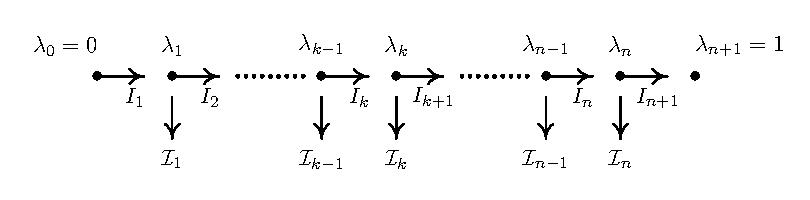
\includegraphics[ ]{NCFig3.eps}
\parbox{4.2in}{\caption{\label{synapses} Configuration of
point input to a dendritic segment of length $h$. Here
$\mathcal{I}_k=g_k(t)(V_k-E_k)$ in the case of synaptic input at
$\lambda_k$ or $\mathcal{I}_k=\mathcal{I}_k(t)$ if the input is an
exogenous point current.}}
\end{figure}

%\begin{figure}[!h]
%\centerline{\qquad\begin{mfpic}[0.9][1]{-50}{400}{-30}{50}
%\pen{1pt}
%\headlen7pt
%%
%% Sealed cable
%\arrow\lines{(0,20),(25,20)}
%\arrow\lines{(40,20),(65,20)}
%\arrow\lines{(120,20),(145,20)}
%\arrow\lines{(160,20),(185,20)}
%\arrow\lines{(240,20),(265,20)}
%\arrow\lines{(280,20),(305,20)}
%%
%%
%\dotspace=4pt
%\dotsize=2pt
%\dotted\lines{(75,20),(110,20)}
%\dotted\lines{(195,20),(230,20)}
%%
%% Nodes on sealed cable
%\tlabel[cc](0,20){\large $\bullet$}
%\tlabel[cc](40,20){\large $\bullet$}
%\tlabel[cc](120,20){\large $\bullet$}
%\tlabel[cc](160,20){\large $\bullet$}
%\tlabel[cc](240,20){\large $\bullet$}
%\tlabel[cc](280,20){\large $\bullet$}
%\tlabel[cc](320,20){\large $\bullet$}
%%
%% Points on sealed cable
%\tlabel[br](0,30){$\lambda_0=0$}
%\tlabel[bc](40,30){$\lambda_1$}
%\tlabel[bc](120,30){$\lambda_{k-1}$}
%\tlabel[bc](160,30){$\lambda_k$}
%\tlabel[bc](240,30){$\lambda_{n-1}$}
%\tlabel[bc](280,30){$\lambda_n$}
%\tlabel[bl](320,30){$\lambda_{n+1}=1$}
%%
%\tlabel[cc](20,10){$I_1$}
%\tlabel[cc](60,10){$I_2$}
%\tlabel[cc](140,10){$I_k$}
%\tlabel[cc](180,10){$I_{k+1}$}
%\tlabel[cc](260,10){$I_n$}
%\tlabel[cc](300,10){$I_{n+1}$}
%%
%% Sealed cable
%\arrow\lines{(40,10),(40,-10)}
%\tlabel[tc](40,-15){\textsf{$\mathcal{I}_1$}}
%\arrow\lines{(120,10),(120,-10)}
%\tlabel[tc](120,-15){\textsf{$\mathcal{I}_{k-1}$}}
%\arrow\lines{(160,10),(160,-10)}
%\tlabel[tc](160,-15){\textsf{$\mathcal{I}_k$}}
%\arrow\lines{(240,10),(240,-10)}
%\tlabel[tc](240,-15){\textsf{$\mathcal{I}_{n-1}$}}
%\arrow\lines{(280,10),(280,-10)}
%\tlabel[tc](280,-15){\textsf{$\mathcal{I}_n$}}
%\end{mfpic}}
%\centering
%\parbox{4in}{\caption{\label{synapses} Configuration of
%point input to a dendritic segment of length $h$. Here
%$\mathcal{I}_k=g_k(t)(V_k-E_k)$ in the case of a synapse at
%$\lambda_k$ or $\mathcal{I}_k=\mathcal{I}_k(t)$ in the case of an
%exogenous input.}}
%\end{figure}

Since distributed current alone can flow across the membrane of a
sub-segment, equation (\ref{mp2}) may be used to describe the
axial current in the $k$-th sub-segment by replacing
$V_\mathrm{P}$ and $r_\mathrm{P}$ with $V_{k-1}$ and $r_{k-1}$
respectively, by replacing $V_\mathrm{D}$ and $r_\mathrm{D}$ with
$V_k$ and $r_k$ respectively, and by replacing $h$ with
$h(\lambda_k- \lambda_{k-1})$, the length of the sub-segment. If
$V_1,\ \cdots\ ,V_n$ are the potentials at the points $\lambda_1,\
\cdots, \lambda_n$ at which point process input is applied, then
the axial currents $I_1,\ \cdots\ , I_{n+1}$ are related to the
potentials $V_1,\ \cdots\ ,V_n$ by the equations
\begin{equation}\label{syn2}
I_k = \ds\frac{\pi g_\mathrm{A}r_{k-1}\,r_k}
{h(\lambda_k-\lambda_{k-1})}\,\big(V_{k-1}-V_k\,\big)\,,\qquad
k=1,\cdots,(n+1)
\end{equation}
where it is understood that $\lambda_0=0$, $\lambda_{n+1}=1$,
$r_0=r_\mathrm{P}$, $r_{n+1}=r_\mathrm{D}$, $V_0=V_\mathrm{P}$ and
$V_{n+1}=V_\mathrm{D}$. Equations (\ref{syn2}) are rearranged in
the form
\[
V_{k-1}-V_k=\frac{h}{\pi g_\mathrm{A}}\,
\frac{(\lambda_k-\lambda_{k-1})}{r_{k-1}\,r_k}
\,I_k \,,\qquad k=1,\cdots,(n+1)\,.
\]
By recognising that $V_k-V_\mathrm{P}$ is the sum of the potential
differences across the first $k$ sub-segments, it follows
immediately from the previous equation that
\begin{equation}\label{syn3}
V_k = V_\mathrm{P} -\frac{h}{\pi g_\mathrm{A}}\,\sum_{j=1}^k \,
\frac{(\lambda_j-\lambda_{j-1})}{r_{j-1}\,r_j}\,I_j \,,\qquad
k=1,\cdots,n\,.
\end{equation}
If $\lambda_k$ is the point of application of an exogenous input
of strength $\mathcal{I}_k(t)$ then
\begin{equation}\label{syn1b}
I_{k+1}+\mathcal{I}_k(t) = I_k\,.
\end{equation}
On the other hand, if there is a synapse at $\lambda_k$, then
$\mathcal{I}_k=g_k(t)(V_k-E_k)$ and conservation of current
requires that
\begin{equation}\label{syn1a}
I_{k+1}+g_k(V_k-E_k) = I_k\,.
\end{equation}
Formula (\ref{syn3}) for $V_k$ is now used to rewrite equation
(\ref{syn1a}) in terms of axial currents to get
\begin{equation}\label{syn4}
I_k-I_{k+1}+\ds\frac{g_k h}{\pi g_\mathrm{A}}\sum_{j=1}^k
\frac{(\lambda_j-\lambda_{j-1})}{r_{j-1}\,r_j}\,I_j =
g_k\big(\,V_\mathrm{P}-E_k\,\big)\,,\qquad k=1,\cdots,n\,.
\end{equation}
Thus conservation of current at the points $\lambda_1,\ \cdots,\
\lambda_n$ gives rise to $n$ equations for the $(n+1)$ currents
$I_1,\ \cdots,\ I_{n+1}$. In order to complete the system of
equations specifying $I_1,\ \cdots,\ I_{n+1}$, note that the
potentials at the proximal and distal boundaries of the segment
are known, and that this condition constrains the currents $I_1,\
\cdots,\ I_{n+1}$ to satisfy
\begin{equation}\label{syn5}
\sum_{j=1}^{n+1}
\frac{(\lambda_j-\lambda_{j-1}) r_\mathrm{P}r_\mathrm{D} }
{r_{j-1}\,r_j}\,I_j =
\frac{\pi g_\mathrm{A}r_\mathrm{P}r_\mathrm{D}}{h}\,
\big(\,V_\mathrm{P}-V_\mathrm{D}\,\big)\,.
\end{equation}
Equation (\ref{syn5}) is obtained from equation (\ref{syn3}) by
asserting that $V_{n+1}=V_\mathrm{D}$. Note also that equation
(\ref{syn5}) has been multiplied by the factor $r_\mathrm{P}
r_\mathrm{D}$ for the benefit of numerical work to make the
coefficients of the currents in the rescaled equation order one.
To summarise, the currents $I_1, \dots I_{n+1}$ are determined by
solving the linear equations
\begin{equation}\label{syn6}
\begin{array}{c}
\left.\begin{array}{rcl}
I_k-I_{k+1} & = &\mathcal{I}_k(t) \,\\
\ds I_k-I_{k+1}+\ds\frac{g_k h}{\pi g_\mathrm{A}}\sum_{j=1}^k
\frac{(\lambda_j-\lambda_{j-1})}{r_{j-1}\,r_j}\,I_j & = &
g_k\big(\,V_\mathrm{P}-E_k\,\big)\,,
\end{array}\right] \qquad k=1,\cdots,n\\[25pt]
\ds\sum_{j=1}^{n+1}
\frac{(\lambda_j-\lambda_{j-1})r_\mathrm{P}r_\mathrm{D}}
{r_{j-1}\,r_j}\,I_j  =
\ds\frac{\pi g_\mathrm{A}r_\mathrm{P}r_\mathrm{D}}{h}\,
\big(\,V_\mathrm{P}-V_\mathrm{D}\,\big)
\end{array}
\end{equation}
where the first equation is used if $\lambda_k$ is the location of
an exogenous point input and the second equation is used if
$\lambda_k$ is the location of a synapse. The following example
illustrates an application of equations (\ref{syn6}) to the case
of a single synapse and a single exogenous input.

\paragraph{Example}
Consider a segment which receives synaptic input of conductance
$g_1(t)$ at $\lambda_1$ and exogenous current $\mathcal{I}_2(t)$
at $\lambda_2$ where $0 < \lambda_1 < \lambda_2 < 1$. This
partitioning of the segment gives rise to three currents $I_1$,
$I_2$ and $I_3$. The determination of $I_\mathrm{P}$ and
$I_\mathrm{D}$ will require expressions for $I_1$ and $I_3$ in
terms of the known conductance $g_1(t)$, the known current
$\mathcal{I}_2(t)$, the geometry of the segment, and finally, the
potentials $V_\mathrm{P}$ and $V_\mathrm{D}$ at the proximal and
distal boundaries of the segment. The formulation of this problem
will involve the current $I_2$ as an auxiliary variable, but the
solution for $I_2$ is not sought. It follows from equations
(\ref{syn6}) that $I_1$, $I_2$ and $I_3$ satisfy
\begin{equation}\label{syn10}
\begin{array}{rcl}
I_1-I_2+\ds\frac{g_1(t) h}{\pi
g_\mathrm{A}}\frac{(\lambda_1-\lambda_0)}{r_0\,r_1}\,I_1 & = &
g_1(t)\big(\,V_\mathrm{P}-E_1\,\big)\,,\\[10pt]
I_2-I_3 & = & \mathcal{I}_2(t)\,,\\[10pt]
\ds\frac{(\lambda_1-\lambda_0)r_0\,r_3}{r_0\,r_1}\,I_1
+\frac{(\lambda_2-\lambda_1)r_0\,r_3}{r_1\,r_2}\,I_2+
\frac{(\lambda_3-\lambda_2)r_0\,r_3}{r_2\,r_3}\,I_3 & = &
\ds\frac{\pi g_\mathrm{A}r_0\,r_3}{h}\,\big(\,V_\mathrm{P}-V_\mathrm{D}\,\big)\,.
\end{array}
\end{equation}
The first equation in (\ref{syn10}) is equation (\ref{syn4})
applied at the location of the synapse ($\lambda=\lambda_1$), and
the second equation in (\ref{syn10}) is equation (\ref{syn1b})
applied at the location of the exogenous current
($\lambda=\lambda_2$). The last equation in (\ref{syn10}) is the
the consistency condition expressed by equation (\ref{syn5}).
Equations (\ref{syn10}) can be expressed in matrix form $AX=B$
where $X=\big[\,I_1,I_2,I_3\,\big]^\mathrm{T}$ and
\[
A=\left[\begin{array}{ccc}
1+\ds\frac{g_1(t) h}{\pi g_\mathrm{A}}\frac{(\lambda_1-\lambda_0)}
{r_0\,r_1} & -1 & 0 \\[10pt]
0 & 1 & -1 \\[10pt]
\ds\frac{(\lambda_1-\lambda_0)r_3}{r_1}
& \ds\frac{(\lambda_2-\lambda_1)r_0\,r_3}{r_1\,r_2}
& \ds\frac{(\lambda_3-\lambda_2)r_0}{r_2}
\end{array}\right],\quad
B=\left[\begin{array}{c}
g_1(t)\big(V_\mathrm{P}-E_1) \\[20pt]
\mathcal{I}_2(t) \\[20pt]
\ds\frac{\pi g_\mathrm{A}r_0\,r_3}{h}\big(V_\mathrm{P}-V_\mathrm{D}\big)
\end{array}\right].
\]
It is a matter of careful algebra to show that the currents $I_1$
and $I_3$ are given by the expressions
\begin{equation}\label{syn11}
\begin{array}{rcl}
I_1 & = & \frac{\ds\frac{\pi g_\mathrm{A}r_0\,r_3}{h}
\big(V_\mathrm{P}-V_\mathrm{D}\big)
+(1-\lambda_1)\frac{r_0}{r_1}g_1(t)\big(V_\mathrm{P}-E_1\big)
+\mathcal{I}_2(t)(1-\lambda_2)\frac{r_0}{r_2}}{\ds 1+
\frac{\lambda_1(1-\lambda_1)hg_1(t)\strut}{\pi
g_\mathrm{A}r_1^2}}\,,\\[35pt]
I_3 & = & \frac{\begin{array}{l}
\ds\frac{\pi g_\mathrm{A}r_0\,r_3}{h} \Big(1+\frac{\lambda_1 h g_1(t)}
{\pi g_\mathrm{A}r_0r_1}\Big) \big(V_\mathrm{P}-V_\mathrm{D}\big)
-\frac{\lambda_1 r_3}{r_1}g_1(t)\big(V_\mathrm{P}-E_1\big)\\[10pt]
\qquad\qquad\ds-\;\mathcal{I}_2(t)\frac{r_3}{r_2}\Big(\lambda_2
+\frac{\lambda_1(\lambda_2-\lambda_1) h g_1(t)}{\pi g_\mathrm{A}
r_1^2}\Big)\end{array}}
{\ds 1+\frac{\lambda_1(1-\lambda_1)hg_1(t)\strut}{\pi g_\mathrm{A}r_1^2}}\,.
\end{array}
\end{equation}
Of course, the complexity of these expressions for $I_1$ and $I_3$
is in part due to the fact that they combine the axial current in
the segment in the absence of point input with the modification to
this current due to the presence of the synaptic input at
$\lambda=\lambda_1$ and the exogenous input at
$\lambda=\lambda_2$. The perturbations
$I_\mathrm{P}=I_1-I_\mathrm{PD}$ and
$I_\mathrm{D}=I_3-I_\mathrm{PD}$ to the axial current at the
proximal and distal boundaries of the segment are now calculated
from formulae (\ref{mp2}) and (\ref{syn11}) to give
\begin{equation}\label{syn12}
\begin{array}{rcl}
I_\mathrm{P} & = & \frac{\ds\frac{r_0(1-\lambda_1)}{r_1}\,
g_1(t)\big(\,\psi_1-E_1\,\big)
+\mathcal{I}_2(t)(1-\lambda_2)\frac{r_0}{r_2}}{\ds 1+
\frac{\lambda_1(1-\lambda_1)hg_1(t)\strut}{\pi
g_\mathrm{A}r_1^2}}\,,\\[35pt]
-\,I_\mathrm{D} & = &
\frac{\ds\frac{\lambda_1 r_3}{r_1}\,g_1(t)\big(\,\psi_1-E_1\,\big)
+\mathcal{I}_2(t)\frac{r_3}{r_2}\Big[\lambda_2+\frac{g_1(t)
h \lambda_1(\lambda_2-\lambda_1)}{\pi g_\mathrm{A}r_1^2}\Big]}
{\ds 1+\frac{\lambda_1(1-\lambda_1)hg_1(t)\strut}{\pi
g_\mathrm{A}r_1^2}}\,.
\end{array}
\end{equation}
where $\psi_1$ is the potential
\begin{equation}\label{syn13}
\psi_1 = \frac{r_0(1-\lambda_1) V_\mathrm{P} + r_3 \lambda_1
V_\mathrm{D}}{r_1}\,.
\end{equation}
It is clear from (\ref{mp3}) that $\psi_1$ would be the model
potential at $\lambda=\lambda_1$ in the absence of transmembrane
current, and therefore $g_1(t)\big(\,\psi_1-E_1\,\big)$ would be
the transmembrane current supplied by the synapse at
$\lambda=\lambda_1$ assuming that this synaptic current is
negligible by comparison with the axial current. Furthermore, if
the common denominator of expressions (\ref{syn12}) is treated as
unity, then expressions (\ref{syn12}) simplify to
\begin{equation}\label{syn14}
\begin{array}{rcl}
I_\mathrm{P} & = & \ds\frac{r_0(1-\lambda_1)}{r_1}\,
g_1(t)\big(\,\psi_1-E_1\,\big)
+\mathcal{I}_2(t)(1-\lambda_2)\frac{r_0}{r_2}\,,\\[10pt]
-\,I_\mathrm{D} & = & \ds\frac{\lambda_1
r_3}{r_1}\,g_1(t)\big(\,\psi_1-E_1\,\big)
+\mathcal{I}_2(t)\frac{r_3}{r_2}\,\lambda_2\,,
\end{array}
\end{equation}
which are identical to equations (\ref{ei1}) with
$\mathcal{I}_1=g_1(t)\big(\,\psi_1-E_1\,\big)$ and
$\mathcal{I}_2=\mathcal{I}(t)$. Expressions (\ref{syn14}) are
those that would follow from making the assumption that
transmembrane current is negligible by comparison with axial
current in the presence of synaptic input. Consequently, the use
of expressions (\ref{syn14}) for $I_\mathrm{P}$ and $I_\mathrm{D}$
would overestimate the true strength of both the synaptic and the
exogenous input to a segment. In conclusion, synaptic and
exogenous input do not act independently when a segment receives
both types of point process input.

The second stage of the analysis deals with the construction and
numerical solution of the equations constructed from the
particular configuration of synapses and exogenous input, and is
given in Appendix 1.

\subsection{Distributed transmembrane current}

All distributed transmembrane current is treated using equations
(\ref{potc3}) with appropriate expressions for $J(\lambda,t)$, and
with occurrences of the membrane potential approximated by
expression (\ref{mp3}). Capacitative current and intrinsic
voltage-dependent current are considered separately.

\subsubsection{Capacitative transmembrane current}\label{CapCurrent}

The component of capacitative current in (\ref{tc2}) is estimated
by approximating the true membrane potential along the segment by
expression (\ref{mp3}) to obtain
\begin{equation}\label{dtc2}
J^\mathrm{\,cap}(\lambda,t)=2\pi
c_\mathrm{M}(\lambda) r(\lambda) \frac{dV(\lambda,t)}{dt} = 2\pi
c_\mathrm{M}(\lambda) \Big[\,(1-\lambda)\,r_\mathrm{P}\,\frac{dV_\mathrm{P}}{dt}
+\lambda\,r_\mathrm{D}\frac{dV_\mathrm{D}}{dt}\,\Big]\,.
\end{equation}
It now follows from expressions (\ref{potc3}) that the
contributions  made by capacitative transmembrane current to
$I_\mathrm{P}$ and to $I_\mathrm{D}$ are
\begin{equation}\label{dtc3}
\begin{array}{rcl}
I^\mathrm{\,cap}_\mathrm{P} & = & 2\pi\, r_\mathrm{P} h
\ds\Big[r_\mathrm{P}\frac{dV_\mathrm{P}}{dt}
\int_0^1\frac{(1-\lambda)^2 c_\mathrm{M}(\lambda)\,d\lambda}
{(1-\lambda)\,r_\mathrm{P}+\lambda\,r_\mathrm{D}}
+r_\mathrm{D}\frac{dV_\mathrm{D}}{dt}
\int_0^1 \frac{\lambda(1-\lambda)c_\mathrm{M}(\lambda)\,d\lambda}
{(1-\lambda)\,r_\mathrm{P}+\lambda\,r_\mathrm{D}}\Big],\\[12pt]
-I^\mathrm{\,cap}_\mathrm{D} & = & 2\pi\, r_\mathrm{D} h
\ds\Big[r_\mathrm{P}\frac{dV_\mathrm{P}}{dt}\int_0^1\,
\frac{\lambda(1-\lambda)c_\mathrm{M}(\lambda)\,d\lambda}
{(1-\lambda)\,r_\mathrm{P}+\lambda\,r_\mathrm{D}}+r_\mathrm{D}
\frac{dV_\mathrm{D}}{dt}\int_0^1\,\frac{\lambda^2
c_\mathrm{M}(\lambda)\,d\lambda}
{(1-\lambda)\,r_\mathrm{P}+\lambda\,r_\mathrm{D}}\,\Big]\,.
\end{array}
\end{equation}
If the compartment is a uniform cylinder with constant specific
membrane capacitance, the perturbations in axial current at the
proximal and distal boundaries of the segment may be computed by
evaluating the integrals in formulae (\ref{dtc3}) to get
\begin{equation}\label{dtc4}
I^\mathrm{\,cap}_\mathrm{P} = \frac{C}{6}\,
\Big[\,2\frac{dV_\mathrm{P}}{dt}+\frac{dV_\mathrm{D}}{dt}\,\Big],
\qquad -I^\mathrm{\,cap}_\mathrm{D} = \frac{C}{6}\,
\Big[\,\frac{dV_\mathrm{P}}{dt}+2\frac{dV_\mathrm{D}}{dt} \,\Big]
\end{equation}
where $C$ is the total membrane capacitance of the segment. The
calculation for tapered segments with non-uniform membrane
specific capacitance is presented in Appendix 2.

\subsubsection{Intrinsic voltage-dependent transmembrane current}

The construction of $I^\mathrm{\,cap}_\mathrm{P}$ and
$I^\mathrm{\,cap}_\mathrm{D}$ for a membrane with non-constant
specific capacitance provides the framework for treating intrinsic
voltage-dependent transmembrane current. For an ionic species
$\alpha$, this current is usually described by the constitutive
formula $J=g_\alpha(\bs{\theta})(V-E_\alpha)$ where $V$ is the
membrane potential, $E_\alpha$ is the reversal potential for
species $\alpha$ and $g_\alpha(\bs{\theta})$ is a membrane
conductance which depends on a set of auxiliary variables
$\bs{\theta}$, for example, the probabilities $m$, $n$ and $h$
appearing in the Hodgkin-Huxley (\cite{Hodgkin52}) model.

In the case of a \emph{passive} membrane, the conductance
$g_\alpha(\bs{\theta})$ takes a constant (but different) value for
each species. The total transmembrane current density is obtained
by summing the transmembrane current densities of each ionic
species to get
\begin{equation}\label{dtc8}
J=\sum_\alpha\, g_\alpha(V-E_\alpha)= g_\mathrm{M}(V-E)\,,
\qquad g_\mathrm{M}=\sum_\alpha g_\alpha\,,\quad
E=\sum_\alpha \frac{g_\alpha}{g_\mathrm{M}}\, E_\alpha\,.
\end{equation}
Thus the constitutive equation for the transmembrane current
density of a passive membrane is $J=g_\mathrm{M}(V-E)$ where
$g_\mathrm{M}$ (mS/cm$^2$) is the total membrane conductance and
$E$ plays the role of a reversal potential. When the segment is a
uniform cylinder with a membrane of constant conductance, the
contributions to $I_\mathrm{P}$ and $I_\mathrm{D}$ mimic formulae
(\ref{dtc4}) for capacitative current and are respectively
\begin{equation}\label{dtc10}
I^\mathrm{\,IVDC}_\mathrm{P} = \frac{G}{6}\,
\Big[\,2(V_\mathrm{P}-E)+(V_\mathrm{D}-E)\Big]\,,\qquad
-I^\mathrm{\,IVDC}_\mathrm{D} = \frac{G}{6}
\Big[\,(V_\mathrm{P}-E)+2(V_\mathrm{D}-E)\Big]
\end{equation}
where $G$ is the total membrane conductance of the segment. The
treatment of tapered segments with non-uniform membrane
conductance is presented in Appendix 3.
